\documentclass[conference]{IEEEtran}
\IEEEoverridecommandlockouts
% The preceding line is only needed to identify funding in the first footnote. If that is unneeded, please comment it out.
\usepackage{cite}
\usepackage{amsmath,amssymb,amsfonts}
\usepackage{algorithmic}
\usepackage{graphicx}
\usepackage{textcomp}
\usepackage{xcolor}
\def\BibTeX{{\rm B\kern-.05em{\sc i\kern-.025em b}\kern-.08em
    T\kern-.1667em\lower.7ex\hbox{E}\kern-.125emX}}
\begin{document}

\title{Multimodal Learning For Human Activity Recognition
}

\author{\IEEEauthorblockN{1\textsuperscript{st} Ravi Raghavan}
\IEEEauthorblockA{\textit{Electrical and Computer Engineering Department} \\
\textit{Rutgers University}\\
New Brunswick, USA \\
rr1133@scarletmail.rutgers.edu}
\and
\IEEEauthorblockN{2\textsuperscript{nd} Abid Azad}
\IEEEauthorblockA{\textit{Electrical and Computer Engineering Department} \\
\textit{Rutgers University}\\
New Brunswick, USA \\
aa2177@scarletmail.rutgers.edu}
}

\maketitle

\begin{abstract}
This paper explores the development of machine learning models for Human Activity Recognition (HAR) using smartphone sensor data. The dataset under investigation is sourced from the UCI repository, capturing the movements of 30 individuals engaged in various activities with smartphones strapped to their waists. The study aims to construct predictive models for six human activities, including Walking, Walking Upstairs, Walking Downstairs, Sitting, Standing, and Lying.

Two distinct phases are employed in the approach: the first utilizing classical machine learning algorithms on a pre-engineered dataset, and the second employing deep learning models on raw sensor data. The hypotheses tested include the performance of logistic regression and linear support vector classifier (SVC) as baseline models, the impact of pre-engineered versus raw datasets, the adaptability of transformer and LSTM models, and the influence of training time on model performance.

The experiments reveal that classical models perform well on pre-engineered datasets, while deep learning models show promise with raw sensor data. The LSTM model's accuracy improves with the number of layers, and the transformer model, despite its complexity, lags behind in performance due to data limitations. The study emphasizes the critical role of data preprocessing, model architecture, and dataset characteristics in designing effective HAR systems.

The findings provide valuable insights for researchers and practitioners in tailoring HAR models to real-world scenarios, taking into account the interplay between model complexity and dataset characteristics.
\end{abstract}

\begin{IEEEkeywords}
LSTM, Transformer, Attention, Multi-Head Attention
\end{IEEEkeywords}

\section{Introduction}

Multimodal Learning in Sensing Systems and Machine Learning for the Internet of Things (IoT) presents novel methods for how we enable devices to understand and interact with the world. In traditional Machine Learning, models are typically unimodal, often using only one form of data such as text or numerical data. However, the advent of IoT has ushered in an era where devices are equipped with diverse sensors, capable of capturing information through various modalities, including visual, auditory, and tactile inputs. \newline 

By leveraging the collective power of these various data sources, Multimodal Learning enables intelligent systems to better interpret and respond to the complexity of real-world environments. This integration of multiple modalities not only enhances the accuracy and robustness of machine learning models but also creates new opportunities for applications ranging from smart homes and healthcare to industrial automation, where a more holistic understanding of the environment is crucial for optimal decision-making and efficiency. \newline 

In the realm of human activity recognition, our research project endeavors to address a pivotal question: How can multimodal learning techniques be effectively employed to enhance the accuracy and versatility of human activity recognition systems in the context of the Internet of Things (IoT)? The overarching problem statement involves the complexities inherent in comprehending human behavior across diverse modalities of sensor data. In our case, we are using accelerometer and gyroscope 
sensor data obtained from a smartphone. \newline 

While traditional activity recognition models often focus on unimodal inputs, the increasing prevalence of IoT devices equipped with multifaceted sensors necessitates a more comprehensive approach. As technology continues to advance, the impact of this work is quite significant. The ability to accurately decipher and interpret human activities through a multimodal lens holds immense significance for applications like smart environments, healthcare monitoring, and personalized assistance systems. By delving into this research question, we aim to contribute novel insights and methodologies that not only push the boundaries of human activity recognition but also align with the evolving landscape of technology, fostering more intelligent and adaptive interactions between humans and the expanding array of IoT-enabled devices. \newline 

Overall, this paper will provide an overview of machine learning models developed for Human Activity Recognition(HAR) using smartphone sensor data. In particular, using accelerometer and gyroscope sensor data from a smartphone, this work was able to develop several machine learning models to classify human activity. 

\section{Related Work}
In recent years, work surrounding Human Activity Recognition(HAR) has picked up pace. The focus has primarily been on leveraging multiple modes of sensor data to enhance accuracy and efficiency of the systems classifying/recognizing human activity. Numerous studies have explored the potential of these sensor technologies in capturing and deciphering intricate human movements. \newline 

The first work we will present is Reyes-Ortiz et al (2016). This work focuses on developing an energy-efficient approach for human activity recognition using smartphones. The key findings of the research include the successful implementation of a smartphone-based activity recognition model with reduced energy consumption, demonstrating the feasibility of using smartphones for real-time activity monitoring. The methodology involves training support vector machine (SVM) classifiers with fixed-point arithmetic representations, showcasing a practical and energy-efficient solution. Results indicate promising classification accuracies for various physical activities. However, the study acknowledges certain limitations, such as the need for a balance between energy efficiency and classification accuracy and potential challenges in handling diverse real-world scenarios. Overall, the paper contributes valuable insights into optimizing smartphone-based activity recognition systems for practical deployment. \newline

Our work will build upon this work by achieving significant results using a limited dataset(i.e. Smartphone Sensor Data from only 30 participants and with only 128 readings in the time series data). This will address one of the limitations of the study by bringing us closer to achieving a balance between energy efficiency and classification accuracy. \newline 

The next work we will present is Ronao and Cho (2016). This work presents quite a unique approach to human activity recognition. This study introduces a novel approach to human activity recognition (HAR) by employing deep convolutional neural networks (convnets) on smartphone accelerometer and gyroscope data. The methodology is characterized by its capacity to automatically extract pertinent and resilient features without intricate pre-processing or manual feature engineering. Notably, the experiments reveal the superiority of convnets over rival methods, achieving remarkable accuracy, especially in discerning intricate activities such as ascending and descending stairs. The investigation delves into the nuances of network architecture, filter size, and learning rate, analyzing their impacts on performance. Results underscore the efficacy of convnets in handling both raw sensor data and additional information from Fast Fourier Transform. While excelling in dynamic activity classification, the study recognizes that Support Vector Machines (SVM) outperform in discerning stationary activities. \newline 

The study also candidly addresses limitations, emphasizing the need for in-depth analysis of automatically derived features and potential enhancements with a more extensive dataset. Overall, this research contributes valuable insights to the realm of HAR, showcasing convnets as a promising avenue with noteworthy accomplishments and avenues for future exploration. \newline 

To improve upon this study, our work will primarily rely upon the attention mechanism to automatically derive features from the time series data. As we studied in class, when creating predictions, an attention layer in neural networks is used to selectively focus on various portions of the incoming data. The attention mechanism gives each input element a distinct weight rather than considering them all identically, enabling the model to prioritize crucial information and disregard unimportant details. This makes the model more effective in tasks involving sequential or structured data by enhancing its capacity to capture long-range dependencies and relationships within the incoming data.

\section{Data/System Description}
Smartphones are indispensable tools in our daily lives, enhancing communication and offering intelligent assistance through advanced technology. With a portable device containing computing capabilities and interconnectivity, smartphones provide application programming interfaces for third-party tools and applications. Beyond communication, they boast features like cameras, GPS, and web browsers, along with embedded sensors such as accelerometers and gyroscopes. These sensors enable the development of applications tailored to users' specific location, movement, and context.

One notable application is Activity Recognition (AR), which involves monitoring a person's actions using a smartphone. The widespread use of smartphones has made them a valuable means of identifying environmental changes based on the data collected by built-in sensors. Notably, sensors like the gyroscope and accelerometer contribute to the device's ability to analyze an individual's state.

Human Activity Recognition (HAR) systems leverage raw sensor data collected from smartphones to analyze and interpret human movements. Various deep learning approaches are employed to develop models that accurately identify different human motions.


With the  prospect of deciphering raw sensor data identify human movement, researchers have aggregated datasets that serve as authoritative repositories of information extracted from sensors embedded in smartphones. One particular dataset we are interested in this paper is the Human Activity Recognition (HAR) dataset from the UCI dataset storehouse. In this repository, data from 30 individuals—referred to as subjects—engaged in various activities with smartphones strapped to their waists is meticulously recorded. The sensors, armed with accelerometers and gyroscopes, capture the nuances of their movements. To add a layer of precision, the experiment is thoughtfully video recorded, allowing for manual labeling of the collected data. \newline 


\textbf{\underline{Training Data:}} \newline
In our research initiative, we compiled a dataset with 9 Inertial Signals, crafting a time series for each in every experiment. With a 50 Hz sampling frequency over a 2.56-second interval, each time series yielded 128 data points. The comprehensive dataset comprises 7,352 samples of raw inertial signal data. Each sample encapsulates 9 Raw Inertial Signals, with each Raw Inertial Signal represented by a time series of 128 points. Regarding feature-engineered data, we obtained 7,352 samples, each containing 561 features. \newline

\textbf{\underline{Test Data:}} \newline
In the same research initiative, we  gathered a dataset of 9 Inertial Signals. Each experiment resulted in a time series for these signals, sampled at 50 Hz over 2.56 seconds, generating 128 data points per series. The raw inertial signal data comprises 2,947 samples, with each sample containing 9 Raw Inertial Signals, and each Raw Inertial Signal represented by a time series of 128 points. Regarding feature-engineered data, we obtained 2,947 samples, each with 561 features.
\newline

Given the density of this particular dataset, the central question guiding this exploration is: Can machine learning models be developed to actively identify and interpret human activity with precision?

\subsection{Objectives/Hypothesis}
The primary objective of this project is to construct a predictive model for human activities, including Walking, Walking Upstairs, Walking Downstairs, Sitting, Standing, and Lying. Leveraging a relatively modest dataset obtained from the Human Activity Recognition (HAR) Dataset in the UCI repository, our approach involves two distinct phases. The first entails employing a pre-engineered dataset and classical machine learning (ML) algorithms to comprehend and predict human activity. Subsequently, we delve into the raw dataset, utilizing deep learning models to glean insights and forecast human activities.

Human activity recognition poses a formidable challenge, requiring effective time series classification. This task involves predicting an individual's movements based on sensor data, traditionally necessitating profound domain expertise and employing signal processing methods to engineer features from raw data—a prerequisite for fitting a machine learning model accurately.

Ultimately, our project addresses a multiclass classification problem wherein the goal is to predict human activities for a given datapoint, each corresponding to one of the six activities mentioned. To achieve this, we explore the utility of four models. As a foundational step, classical machine learning models such as Logistic Regression and Linear SVC are employed to establish a baseline understanding of the dataset's classifiability using conventional approaches. Subsequently, we aim to enhance the performance benchmarks set by these models by integrating deep learning techniques, specifically Transformers and LSTMs with varying layers.

In formulating our approach, several hypotheses emerge:

\begin{enumerate}

  \item \textbf{Hypothesis on Dataset Impact:}
   \begin{itemize}
      \item The pre-engineered dataset, being tailored for classical ML algorithms, may yield satisfactory results in terms of accuracy.
      \item The raw dataset, with its unprocessed sensor data, may present challenges in feature extraction but holds the promise of capturing more intricate patterns, potentially leading to enhanced performance once processed by deep learning models.
   \end{itemize}

  \item \textbf{Hypothesis on Model Adaptability:}
   \begin{itemize}
      \item Transformers, known for their effectiveness in sequential data tasks, might struggle to demonstrate their full potential within the limited training timeframe and data.
      \item Classical models, being less complex, may adapt more readily to the time constraints, showcasing consistent performance.
   \end{itemize}

\end{enumerate}

Considering these hypotheses, it appears important to conduct a more comprehensive exploration of the dataset, delving into a detailed analysis, and further contemplating strategies for effective data engineering.

\subsection{Feature Selection and Engineering}

\begin{figure}[h!]
	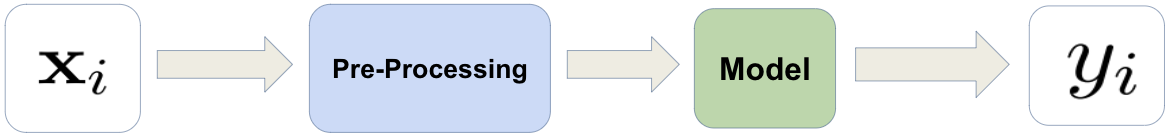
\includegraphics[width= 0.9 \linewidth]{ML Pipeline.png}
	\centering
	\caption{Machine Learning Pipeline}
	\label{ML Pipeline.png}
\end{figure}

As shown by Figure 1, our Machine Learning pipeline resembles a conventional ML Pipeline. First, we receive our input data, which in our case is raw time series data corresponding to accelerometer and gyroscope sensor readings. Then, the aforementioned data is pre-processed and subsequently passed through the Machine Learning Model. Finally, given the output, our system is able to make a prediction regarding the human activity that the data corresponds to. 

In this section, we will be focusing on the Preprocessing Block. We will describe how the preprocessing was done for both the Baseline models and for the Deep Learning Models  

\subsubsection{Baseline Models}

\begin{figure}[h!]
	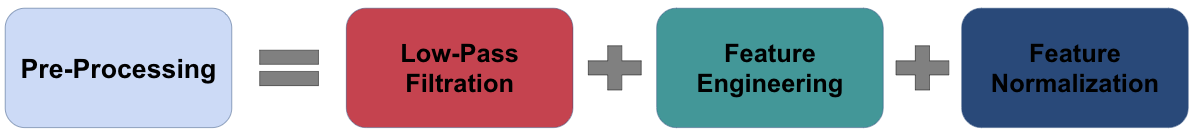
\includegraphics[width= 0.9 \linewidth]{Preprocessing.png}
	\centering
	\caption{Preprocessing}
	\label{Preprocessing.png}
\end{figure}

Figure 2 encapsulates the Preprocessing block used for baseline machine learning models that we used.

\textbf{\underline{Low Pass Filtration}} \newline 
This section entails the low pass filtration which essentially used a 1st Order Butterworth low-pass filter to separate accelerometer sensor data into body acceleration and gravitational components. This is a very common signal processing technique. The purpose is to filter out the high-frequency noise and fast variations in the accelerometer signal, leaving behind the slower-changing gravitational component. \newline 

Let us explain the reasoning behind this. Accelerometer data typically includes both the gravitational acceleration and the body acceleration due to motion. The gravitational component is a constant acceleration vector pointing towards the Earth, while the body acceleration varies based on movement. The body acceleration can vary based on the activity that the test subject. \newline 

A low-pass filter allows low-frequency components to pass through while attenuating higher frequencies. In this project, we chose the cutoff Frequency of the Butterworth Low-Pass Filter to be 0.3 Hz. \newline 

The filtered output represents the gravitational acceleration component. To isolate the body component, we can subtract the graviational acceleration signal from the raw accelerometer data. The result will  represent the body acceleration. \newline 

\textbf{\underline{Feature Engineering}} \newline 
Once we have isolated the gravitational and body acceleration components, we perform Feature Engineering. \newline 

For feature engineering, we will be estimating statistical properties from the body/total acceleration signals and the gyroscope signals. Here are a few examples of statistical properties that were used:
\begin{itemize}
    \item mean(): Mean value
    \item std(): Standard deviation
    \item mad(): Median absolute deviation 
    \item max(): Largest value in array
    \item min(): Smallest value in array
    \item sma(): Signal magnitude area
    \item energy(): Energy measure. Sum of the squares divided by the number of values. 
    \item iqr(): Interquartile range 
    \item entropy(): Signal entropy
    \item arCoeff(): Autorregresion coefficients with Burg order equal to 4
    \item correlation(): correlation coefficient between two signals
    \item maxInds(): index of the frequency component with largest magnitude
    \item meanFreq(): Weighted average of the frequency components to obtain a mean frequency
    \item skewness(): skewness of the frequency domain signal 
    \item kurtosis(): kurtosis of the frequency domain signal 
    \item bandsEnergy(): Energy of a frequency interval within the 64 bins of the FFT of each window.
    \item angle(): Angle between to vectors.
\end{itemize}

\textbf{\underline{Feature Normalization}} \newline 
All features were normalized to be between -1 to 1. \newline 

\subsubsection{Deep Learning Models}
For the Deep Learning models, we used raw acceleration and gyroscope sensor data as input into the deep learning model. We did not do the Feature Engineering because, as we learned in class, neural networks, especially deep learning models, are capable of learning hierarchical representations from raw data. By providing raw signals, the network can automatically learn relevant features and representations at different levels of abstraction.

\subsection{Multimodal Data Patterns}
Prior to doing any pre-processing or machine learning work, the first phase of our project was EDA[Exploratory Data Analysis]. 

\begin{figure}[h!]
	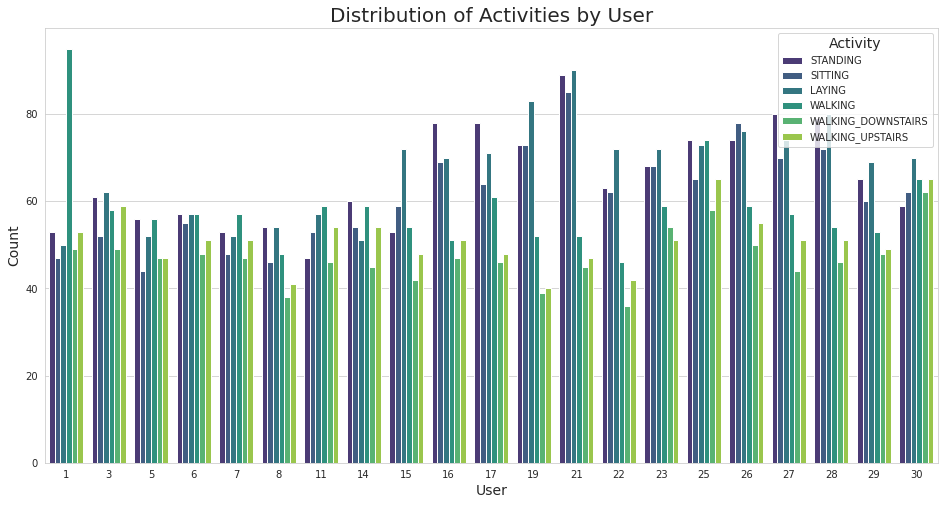
\includegraphics[width= 1.0 \linewidth]{activity_distribution.png}
	\centering
	\caption{Distribution of Activities among Training Experimental Subjects}
	\label{activity_distribution.png}
\end{figure}

Figure 3 shows the distribution of activities among training experimental subjects. The dataset reveals a notable trend wherein participants have a greater volume of data for walking upstairs compared to walking downstairs. Assuming an equal distribution of both uphill and downhill walks, it becomes evident that participants spend a longer duration walking upstairs. \newline 

How is the distribution of activity occurrences in this dataset precisely characterized? Let's generate a plot and delve into the analysis.

\begin{figure}[h!]
	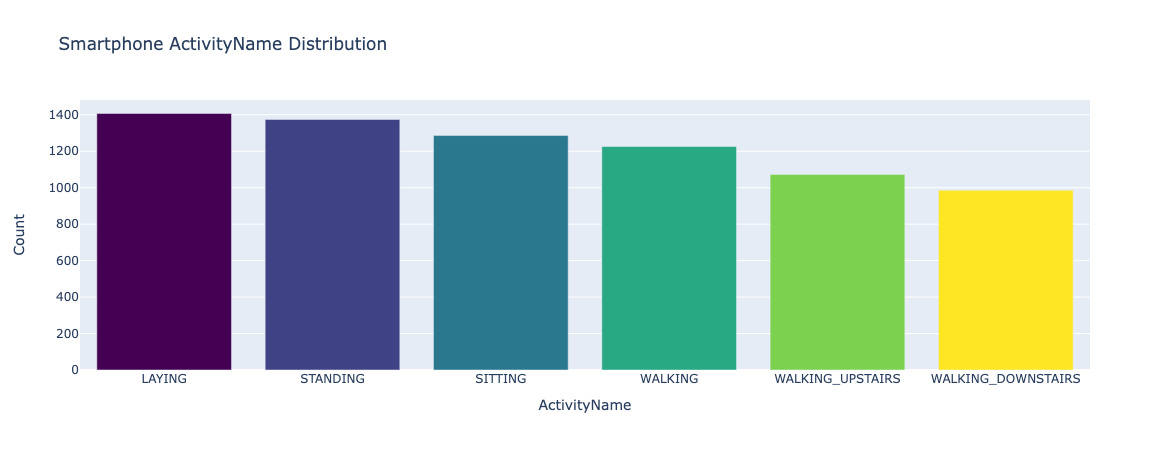
\includegraphics[width= 1.0 \linewidth]{smartphone_activity_name_distribution.png}
	\centering
	\caption{Smartphone Activity Name Distribution}
	\label{smartphone_activity_name_distribution.png}
\end{figure}

Despite fluctuations in label counts, the distribution of labels remains fairly even. Assuming participants ascended and descended an equal number of stairs while smartphones maintained a consistent sampling rate, the dataset should reflect an equal number of data points for both upward and downward walking. Setting aside the potential for flawed data, participants appear to walk approximately 10\% faster when descending. \newline 


Upon initial observation, it is apparent that static activities may not yield as much information as their dynamic counterparts. To substantiate this assertion, let's employ a visual aid for clarification. \newline 

\begin{figure}[h!]
	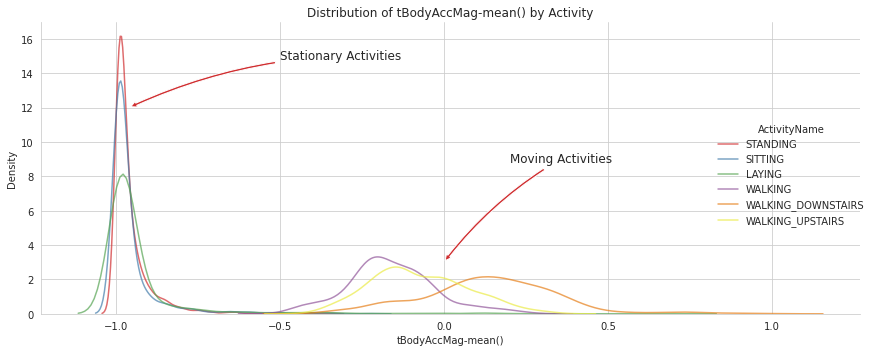
\includegraphics[width= 1.0 \linewidth]{distribution_acc_activity.png}
	\centering
	\caption{Distribution of the Magnitude of Body Acceleration Component}
	\label{distribution_acc_activity.png}
\end{figure}

Explanation of Above Graph: \newline 
\begin{itemize}
    \item The first thing to keep in mind that features in $X\_train.txt$ are normalized and bounded within [-1,1].
    \item Now, let's look at the variable we are analyzing. tBodyAccMag-mean() is the mean magnitude of the body acceleration in the time domain. 
    \item So, at the "-1" end of the graph, this would correspond to a mean magnitude of 0. As we go rightward, this would correspond to an increase in the  mean magnitude of the body acceleration
    \item We can see that, for stationary data, the mean magnitude of body acceleration is roughly 0. This would correspond to expectations
    \item We can see that, for motional data, the mean magnitude of body acceleration is more than 0. This would correspond to expectations. 
\end{itemize}


In real-world datasets, what is often observed is that the distribution of data during participants' movement tends to follow a normal distribution, albeit with some notable long tails. Notably, the magnitude of dynamic activities is significantly higher than that of stationary activities.  \newline 

Now, let's develop a better visual of the distribution of data amidst the activities. \newline 

\begin{figure}[h!]
	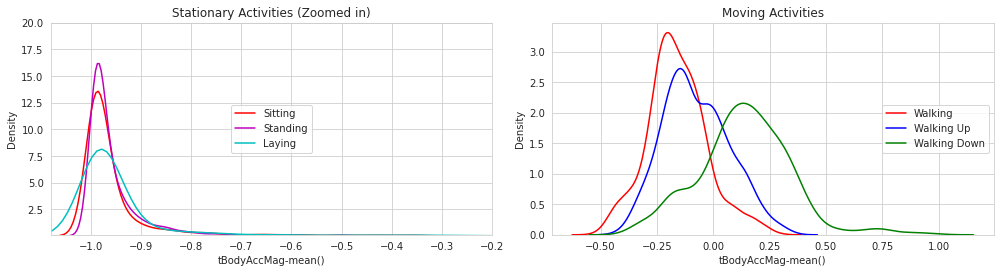
\includegraphics[width= 1.0 \linewidth]{zoomed_distribution_acc_activity.png}
	\centering
	\caption{Zoomed In Distribution of the Magnitude of Body Acceleration Component}
	\label{zoomed_distribution_acc_activity.png}
\end{figure}

The visualizations distinctly illustrate the distribution patterns between Stationary Activities and Moving Activities. Now, the challenge is to precisely differentiate between these activities. One potential approach is to leverage the Magnitude of acceleration as a discriminating factor. To explore this, let's apply a boxplot to visualize and compare the activities.

\begin{figure}[h!]
	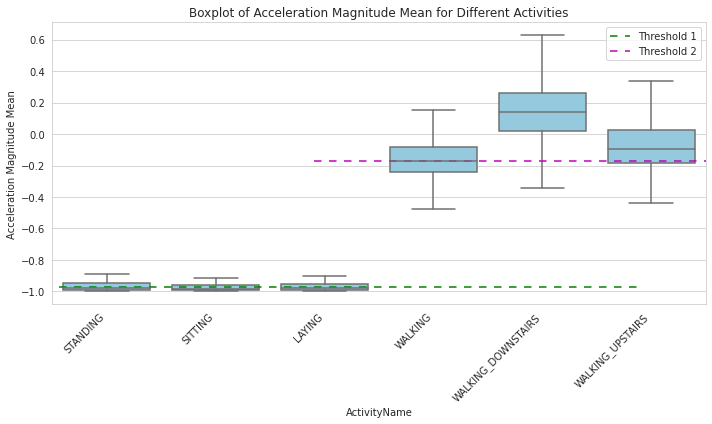
\includegraphics[width= 1.0 \linewidth]{boxplot_acc_magnitude_mean.png}
	\centering
	\caption{Boxplot of Acceleration Magnitude Means}
	\label{boxplot_acc_magnitude_mean.png}
\end{figure}

Analyzing the nuanced patterns unveiled by the box plot reveals valuable distinctions. A tAccMean below -0.8 predominantly corresponds to stationary activities like Standing, Sitting, or Laying. Conversely, when tAccMean exceeds -0.6, it signals dynamic activities such as Walking, Walking Downstairs, or Walking Upstairs. Moreover, a tAccMean surpassing 0.0 specifically characterizes the activity as Walking Downstairs.

While achieving a commendable 75\% classification accuracy for activity labels, there remains a margin for error. It is important to note that threshold lines were strategically added to divide the data, providing a clearer view of the distinctions between activity categories. The consideration of Gravity Acceleration Components adds an additional layer of relevance to the classification task. Thus, revisiting the plots with respect to these components may yield further insights.

\begin{figure}[h!]
	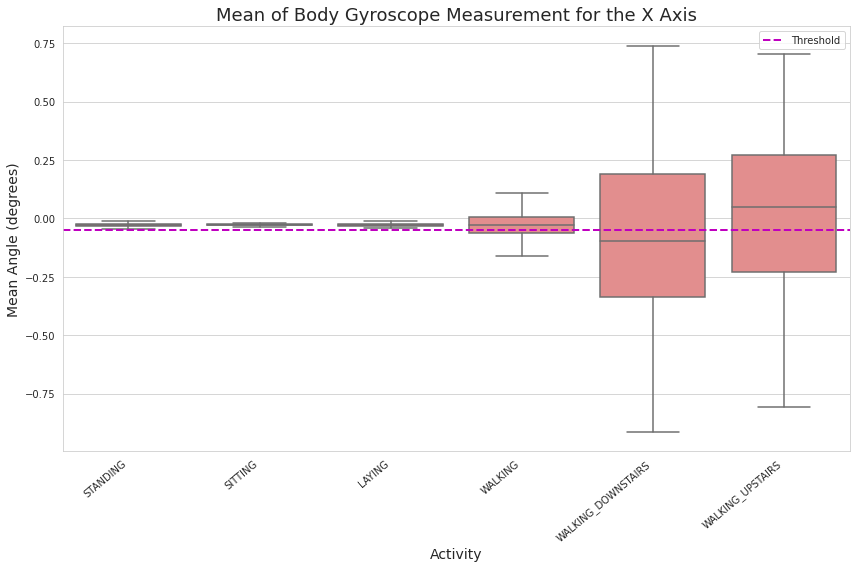
\includegraphics[width= 1.0 \linewidth]{mean_body_gyroscope_x.png}
	\centering
	\caption{Mean of Body Gyroscope Measurement for X Axis}
	\label{mean_body_gyroscope_x.png}
\end{figure}

\begin{figure}[h!]
	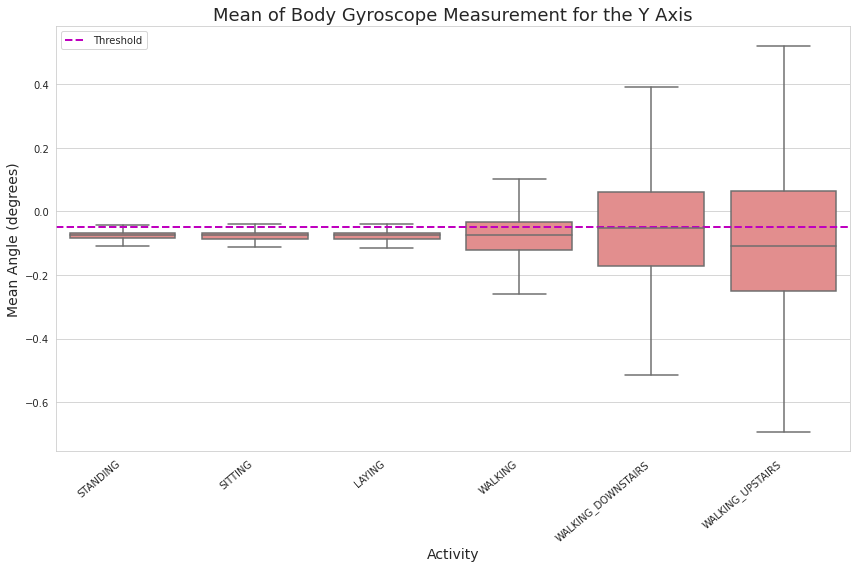
\includegraphics[width= 1.0 \linewidth]{mean_body_gyroscope_y.png}
	\centering
	\caption{Mean of Body Gyroscope Measurement for Y Axis}
	\label{mean_body_gyroscope_y.png}
\end{figure}

\begin{figure}[h!]
	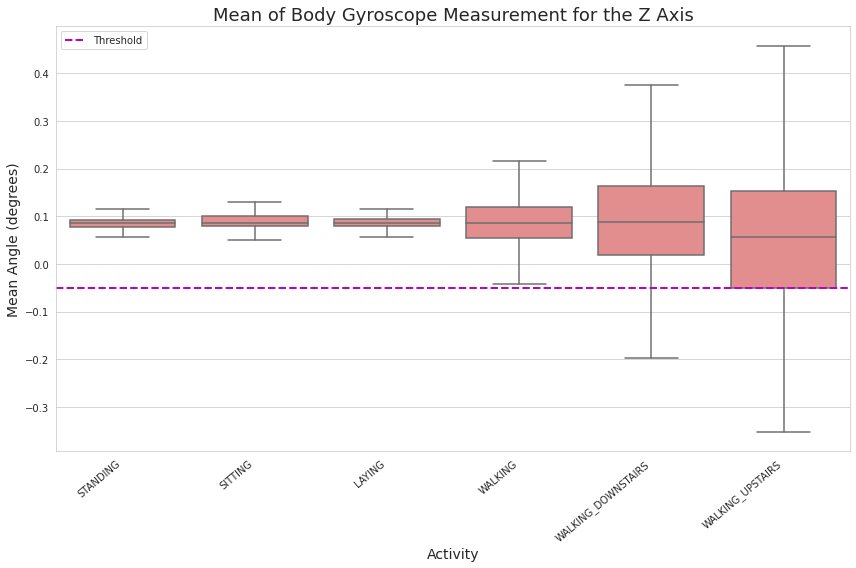
\includegraphics[width= 1.0 \linewidth]{mean_body_gyroscope_z.png}
	\centering
	\caption{Mean of Body Gyroscope Measurement for Z Axis}
	\label{mean_body_gyroscope_z.png}
\end{figure}

The aforementioned gyroscope data clearly shows that there are distinctions in the gyroscope sensor readings among Stationary Activities(i.e. Standing, Sitting, and Laying) versus Motion Activities(i.e. Walking, Walking Upstairs, and Walking Downstairs). This makes perfect sense! Gyroscopes measure angular velocity, which is the rate of rotation. When stationary, the angular velocity is essentially zero, resulting in a relatively stable gyroscope output. This is true because when the gyroscope is stationary, it is affected only by the Earth's gravity. In contrast, when in motion, additional inertial forces come into play, affecting the gyroscope's behavior. Hence, during motion, the gyroscope detects changes in angular velocity, leading to dynamic readings.


\section{Methodology}
In this work, we used the following Machine Learning models: Logistic Regression, Linear Support Vector Classifier(SVC), LSTM(multiple architectures were experimented with), and a Transformer-based model. The Logistic Regression and Linear SVC Models were used as baselines to enable us to compare the performance of the LSTM and Transformer models. \newline 

%Ill fetch the images later.
\textbf{Logistic Regression}: 
Logistic Regression serves as a baseline model, providing insights into the classification task. This linear model, widely employed for binary and multiclass classification, models probabilities using a logistic (sigmoid) function. The logistic function ensures that predictions fall within the range of 0 to 1, making it particularly suitable for classification problems.

We initiated our experiment by fetching and processing data from the Human Activity Recognition (HAR) dataset. Our preprocessing steps involved loading the feature names, training, and testing data. The dataset was divided into singular modality analysis and multimodal analysis, with a subset of features selected for singular modality.

For singular modality analysis, we focused on specific features ('tBodyAcc-mean()-X', 'tBodyAcc-mean()-Y', 'tBodyAcc-mean()-Z') and applied Principal Component Analysis (PCA) to capture 99\% of the variance in the data. \newline 

\underline{Principal Component Analysis}: During our PCA exploration, we started with the original set of engineered features which amounted to 561 features. After conducting PCA, we were able to reduce the number of features to 155. 


The singular modality logistic regression model was then trained on this subset. In the multimodal analysis, the entire set of features was considered. We applied PCA to reduce dimensionality, maintaining 99\% variance. The logistic regression model was trained on this reduced feature set.

To prevent overfitting, we employed L2 regularization (ridge regularization) during the logistic regression model training. Hyperparameter tuning was conducted using grid search with cross-validation to find optimal values for the regularization factor (C) and penalty (l2 or l1).

The trained models were evaluated on the testing dataset, and performance metrics such as accuracy and confusion matrices were computed. Additionally, classification reports were generated to provide a detailed breakdown of the model's performance across different classes.

As a result, the singular modality Logistic Regression model achieved an accuracy of approximately 20.63\% whilst the multimodal Logistic Regression model achieved a significantly higher accuracy of approximately 95.62\%, which , suggests that combining information from a broader set of features, represented by the entire feature set, contributes substantially to the model's ability to accurately classify human activities.


\textbf{Linear SVC}: 
Linear Support Vector Classifier (Linear SVC) serves as a second base line model, offering insights into Human Activity Recognition through classification. Linear SVC aims to find the best-fit hyperplane that separates the data into distinct classes. This hyperplane, once determined, enables the classification of new observations based on their features.

The Linear SVC model follows the same procedure as the Logistic Regression model in terms of setting up the data, creating a singular and multimodal model for analysis, and the reduction of dimensionality through PCA.

Once again, as a reminder \newline 
\underline{Principal Component Analysis}: During our PCA exploration, we started with the original set of engineered features which amounted to 561 features. After conducting PCA, we were able to reduce the number of features to 155. 


The Linear SVC models are then trained on both singular modality and multimodal data. Hyperparameter tuning is conducted using GridSearchCV with cross-validation to find the optimal regularization parameter (C). The tolerance parameter is set to 0.00005 to control the convergence criteria.

As per the other baseline model, trained models are evaluated on the testing dataset, and accuracy metrics are calculated. Additionally, confusion matrices provide insights into the model's performance across different activity classes.

As a result, the singular modality Logistic Regression model achieved an accuracy of approximately 21.99\% whilst the multimodal Logistic Regression model achieved a significantly higher accuracy of approximately 96.20\%, which , suggests that combining information from a broader set of features, represented by the entire feature set, contributes substantially to the model's ability to accurately classify human activities. \newline 

\textbf{LSTM:} Based on the nature of this problem, we deemed the LSTM as an integral portion of our system. As we learned in class, Long Short-Term Memory (LSTM) networks are a type of recurrent neural network (RNN) that are well-suited for sequences of data. Since the raw data we have are accelerometer and gyroscope sensor data, this naturally led us towards the LSTM as a key component of our model architecture. Since accelerometer and gyroscope data are inherently sequential data sources, which represent changes in motion over time, we felt that LSTMs would be best to capture dependencies and patterns in our data. 

Additionally, since LSTMs have the ability to capture and retain information over long sequences, we felt that this was very important for understanding complex human activities that dynamically evolve over time.


\begin{figure}[h!]
	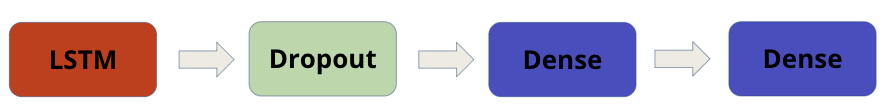
\includegraphics[width= 0.9 \linewidth]{LSTM(1).png}
	\centering
	\caption{LSTM Model Architecture 1}
	\label{LSTM(1).png}
\end{figure}

\begin{figure}[h!]
	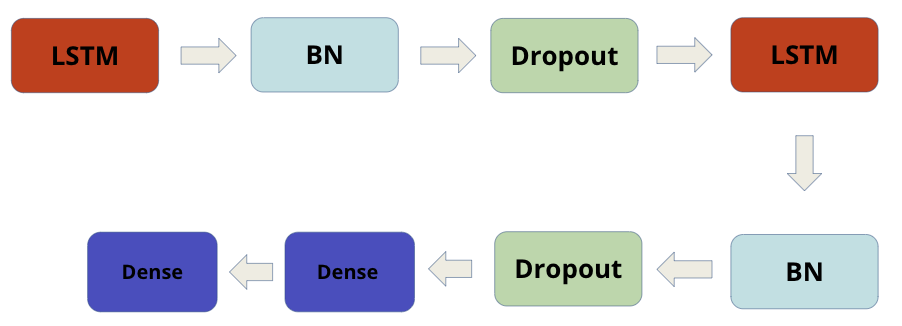
\includegraphics[width= 0.9 \linewidth]{LSTM(2).png}
	\centering
	\caption{LSTM Model Architecture 2}
	\label{LSTM(2).png}
\end{figure}


\begin{figure}[h!]
	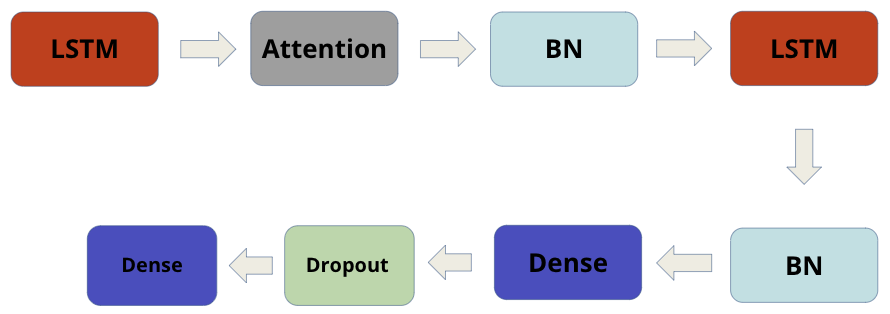
\includegraphics[width= 0.9 \linewidth]{LSTM(3).png}
	\centering
	\caption{LSTM Model Architecture 3}
	\label{LSTM(3).png}
\end{figure}

Here are the three LSTM Model Architectures that we experimented with. Let us dive into each LSTM Model Architecture. 

\textbf{\underline{LSTM Model Architecture 1}} \newline 
This is the first LSTM Model Architecture that we experimented with. Given the input data, the LSTM Layer returned an output vector of size 32. Then, we used a Dropout Layer where 50 percent of the inputs were dropped. Finally, we had two Dense Layers at the end. The first Dense layer outputs a vector of size 16. The activation function for this Dense Layer is ReLU. The second Dense layer outputs a vector of size 6. The activation function for this Dense is softmax \newline 

Now that the architecture has been described, let's dive into the analysis. As discussed previously, the LSTM Layer was included due to its ability to capture and retain information over long sequences. Now, let's discuss the Dropout layer. In each forward pass of training, the Dropout Layer randomly sets some neurons to 0. In this case, since the dropping rate is equal to 0.50, the Dropout Layer will randomly set the output of 50 percent of the neurons to 0 during the training phase. The reason Dropout Layers are effective is quite intuitive. In a hidden layer, when hidden units are trained together, they may co-adapt to the training data. In other words, the weights of one hidden unit may rely on another hidden unit within the same layer. This may make it more difficult for the model to generalize to new test data. \newline 

If a hidden unit has to work well with different combination of other hidden neurons, it will optimize itself to be useful. Each time we present a training batch, we randomly omit each hidden unit with probability equal to the dropping rate. Essentially, we are randomly sampling from a large number of different architectures. Ensembling these different architectures together can achieve improvement in performance \newline 

 
\textbf{\underline{LSTM Model Architecture 2}} \newline 
Adding more LSTM layers increases the overall model complexity. Our human activity recognition task requires a more sophisticated representation of temporal dependencies. Hence, having additional LSTM layers may help the model capture and learn intricate patterns within the data. \newline 

Additionally, we thought to add a Batch Normalization layer whose main idea is to normalizes the input of a layer by subtracting the mean and dividing by the standard deviation of that mini-batch. The normalization is applied independently to each feature (or channel) of the input. We felt that the BatchNorm layer would be useful for an LSTM model that takes accelerometer data and gyroscope data as input. \newline 

The raw accelerometer and gyroscope data have varying ranges. The BatchNorm layer will help normalize these inputs within each mini-batch during training. Normalizing the inputs ensures that the model is less sensitive to the scale of the input features, which will help to improve convergence and training stability. This will also help to make the loss landscape more uniform due to the fact that the BatchNorm layer has made our features on the same scale. \newline 

\textbf{\underline{LSTM Model Architecture 3}} \newline 
An important thing to notice about this model architecture is we incorporated an attention layer. As we learned in the course, the purpose of an attention layer in neural networks is to selectively focus on different parts of the input data when making predictions. Instead of treating all input elements equally, the attention mechanism assigns different weights to them, allowing the model to prioritize important information and ignore irrelevant parts. This helps improve the model's ability to capture long-range dependencies and relationships within the input data, making it particularly useful in tasks involving sequential or structured data. \newline 

We believed that incorporating an attention layer within our model architecture would be useful because it would allow the model to focus on specific time steps or intervals, capturing relevant temporal context for recognizing human activities. Furthermore, since we have tri-axial accelerometer and gyroscope data, we believed that having an attention layer would enable the model to assign different weights to different sensor readings, emphasizing crucial information and downplaying less relevant data. \newline 

Here is a brief mathematical description of how an Attention Layer works: \newline 

Normally, we would have three sequences be passed into an Attention Layer. We have a Query $Q \in \mathbb{R}^{t \times d}$, a Key $K \in \mathbb{R}^{t \times d}$, and a Value $V \in \mathbb{R}^{t \times d}$. In our case, since we are performing self-attention, $Q = K = V$. \newline 

$Attention(Q, K, V) = softmax(\frac{Q (K^T)}{\sqrt{d}}) V \in \mathbb{R}^{t \times d}$ \newline 

Based on these equations here, it is clear to see that the attention mechanism enables the model to assign different weights to different parts of the input sequence, emphasizing more on the relevant components while downplaying less relevant ones. We felt that this would be particularly useful in time series data where certain time steps may contain critical information for the classification task. \newline 


In our implementation, we extended this concept to implement a Multi-Head Attention Layer. The mathematical concepts behind the Multi-Head attention layer have described, in more detail, in section 5.4. Please refer to that for the more-detailed description! \newline 

\textbf{\underline{Transformer}} \newline 
The main reason why we were drawn to the Transformer model was the attention mechanisms within the Transformer model. Transformers employ attention mechanisms that allow the model to focus on different parts of the input sequence when making predictions. This is particularly beneficial for our Human Activity Recognition task, as certain parts of a sequence may be more relevant for recognizing specific activities. The attention mechanism helps the model dynamically weigh the importance of different time steps. Additionally, Transformers, via their attention mechanisms, are really adept in capturing long-range dependencies. \newline 

\begin{figure}[h!]
	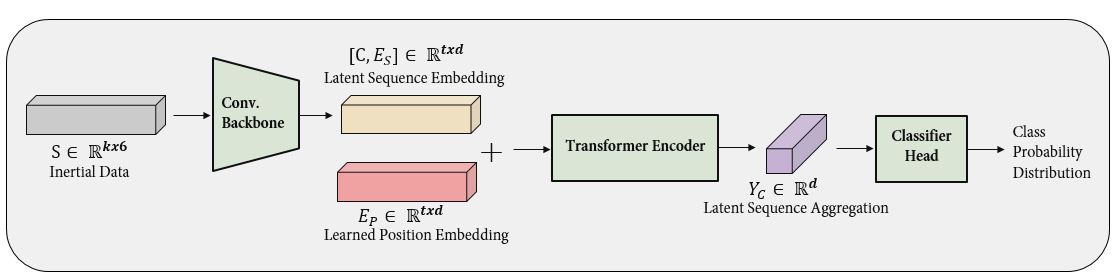
\includegraphics[width= 0.9 \linewidth]{imu_model.png}
	\centering
	\caption{Transformer Model}
	\label{imu_model.png}
\end{figure}

In developing the architecture of the Transformer model, we found a research paper, Reference [1], which had implemented a Transformer based model for Human Activity Recognition based on Inertial-Based Human Activity. Since our research questions also poses similar questions, we decided to implement the model from this paper to see if we could achieve similar results on our dataset! \newline 

The Transformer Model architecture shown in Figure 17 was an idea taken from Reference [1]. The input is \underline{\textbf{Inertial Data}} which is a matrix of size $\mathbb{R}^{k \times 6}$. In our project case, since we had a total of 9 inertial signals, the input would be of size $\mathbb{R}^{k \times 9}$. \newline 

The next step is to take the Raw Inertial Samples and Embed them in a Higher Dimension. To achieve this, we pass the raw inertial samples through a series of four 1D convolutions that are applied with GELU(Gaussian Error Linear Unit) non-linearity. The end-result of this was to embed the raw data in a higher dimension $d$. \newline 


In our opinion, we thought that this would be very useful as embedding time series data in higher dimensions would allow for a more expressive representation of the underlying patterns and structures in the data. These complex relationships and dependencies may not be apparent in lower dimensions. Furthermore, higher dimensional embeddings would be very useful in capturing non-linear relationships in the time series data. \newline 

Overall, the size of the output of this layer(i.e. $E_S$) should be $\mathbb{R}^{k \times d}$. Let $C \in \mathbb{R}^{d}$ represent a class token that is prepended to $E_S$. Additionally, we learn an embedding $E_{P_i} \in \mathbb{R}^d$ for each Position $P_i$ in the sequence $E_S$. 


$Z_0 = [C, E_S] + E_P \in \mathbb{R}^{t \times d}$
where $t = k + 1$ .  

In our implementation, $d = 64$. Additionally, we can treat $Z_0$ as the input to the Transformer Encoder. \newline 

\textbf{\underline{Transformer Encoder}} \newline 
The Transformer Encoder is comprised of $L$ layers each of which are comprised of a Multi-Head Attention unit followed by a Feedforward Neural Network. The Feedforward Neural Network has dimension of $2d$ with GELU(Gaussian Error Linear Unit) Non-linearity. \newline 

In our implementation, we had 6 Transformer Encoder Layers where each Transformer Encoder Layer had a Multi-Head Attention unit with 8 Heads. \newline 

\textbf{\underline{Multi-Head Attention}} \newline
Normally, we would have three sequences be passed into a Multi-Head Attention Layer. We have a Query $Q \in \mathbb{R}^{t \times d}$, a Key $K \in \mathbb{R}^{t \times d}$, and a Value $V \in \mathbb{R}^{t \times d}$ \newline 

$h(Q, K, V) = softmax(\frac{Q_h (K_h^T)}{\sqrt{d}}) V_h \in \mathbb{R}^{t \times d'}$ where \newline

$Q_h = QW_h^Q \in \mathbb{R}^{t \times d'}$ \newline 
$K_h = KW_h^K \in \mathbb{R}^{t \times d'}$ \newline 
$V_h = VW_h^V \in \mathbb{R}^{t \times d'}$ \newline 

where $d' = \frac{d}{n_h}$ and $n_h$ represents the number of heads in the Multi-Head Attention Layer. In our case, $n_h = 8$ and $d = 64$. Hence, $d' = 8$. Evidently, we can treat the matrices $W_h^Q, W_h^K, W_h^V \in \mathbb{R}^{d \times d'}$ as linear projections from the $d$ dimensional space to the $d'$ dimensional space. When we use multi-head attention, we will concatenate the output from each "head" along the channel dimension(i.e. $d$). \newline 

Note: In our case, since we are using self-Multi Head Attention, $Q, K, V$ would all represent the same input sequence! \newline 

To summarize each Transformer Encoder Layer, for $l = 1, 2, 3, ..., L$, we can view it as a two step operation: 
\begin{itemize}
    \item $Z_l ' = sMHA(LN(Z_{l-1})) + Z_{l - 1} \in \mathbb{R}^{t \times d}$
    \item $Z_l = MLP(LN(Z_{l} ')) + Z_{l} ' \in \mathbb{R}^{t \times d}$
\end{itemize}

Note: $sMHA$ represents "self Multi Head Attention", $LN$ represents Layer Normalization, and $MLP$ represents Multi-Layer Perceptron. \newline 

Just as a review, Layer Normalization entails that we perform normalization across the features, independently for each sample. On the other hand, Batch Normalization entails that we perform normalization across the mini-batch, independently for each feature. \newline 


To get the output of the Transformer Encoder Layer, we take $Y_C = Z_L[0] \in \mathbb{R}^d$ \newline

\textbf{\underline{Classification Head}} \newline 
$Y_C$ is provided as input to the Classification Head. First a Layer Normalization is done. Then, we do a Dense Layer with an output size of $d/4$. Then, we do a GELU(Gaussian Error Linear Unit) Non-Linear Activation. Then, we do a Dropout Layer with 10 percent of the nodes dropped out. Finally, we do a Dense Layer with an output of 6 since we have 6 output classes in our system. 

\section{Results}
\begin{figure}[h!]
	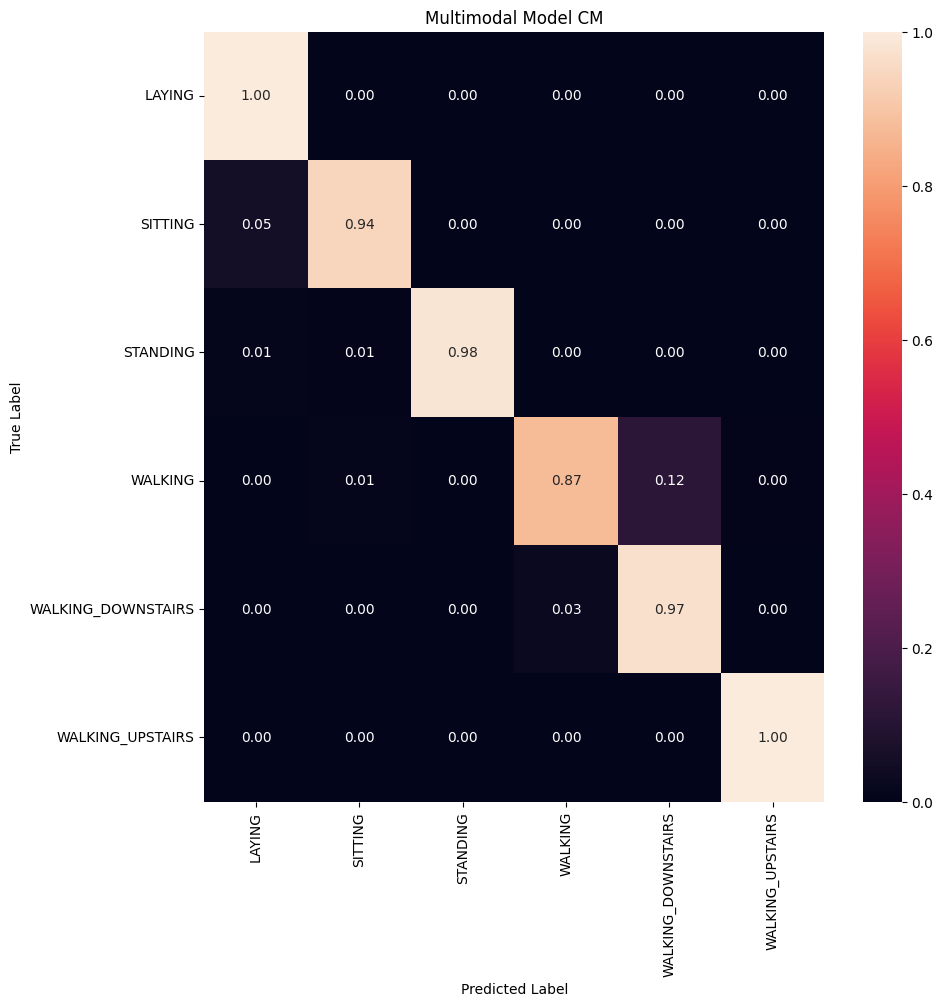
\includegraphics[width= 0.9 \linewidth]{linearSVC.png}
	\centering
	\caption{Linear SVC Results}
	\label{linearSVC.png}
\end{figure}
In reference to Figure 14, portraying the Confusion Matrix for the Linear SVC Model, it becomes apparent that the performance of this architecture is remarkably high. Notably, the model exhibits an outstanding ability to differentiate activities, with only an exceedingly rare occurrence of confusion between Standing and Sitting Down. This infrequent misclassification is understandable given the inherent similarity in sensor readings during these stationary activities. Beyond this rare instance, the model consistently demonstrates precise identification across all other categories.

\begin{figure}[h!]
	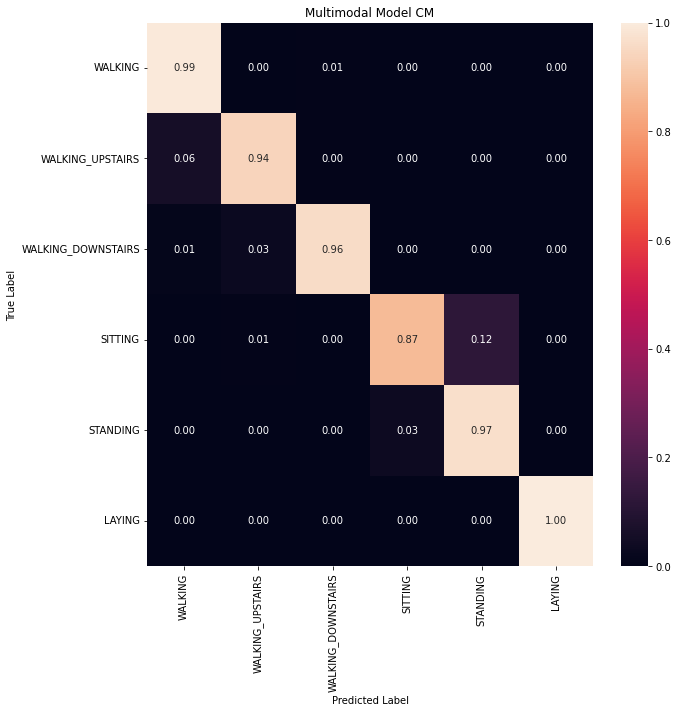
\includegraphics[width= 0.9 \linewidth]{logisticRegression.png}
	\centering
	\caption{Logistic Regression Results}
	\label{logisticRegression.png}
\end{figure}
The examination of the Confusion Matrix Model for Logistic Regression in Figure 16 reveals consistent results, indicating that the data exhibits linear separability and performs exceptionally well under models of this nature. In summary, our baseline models demonstrate effective performance, establishing themselves as valuable benchmarks for our deep learning models.
\begin{figure}[h!]
	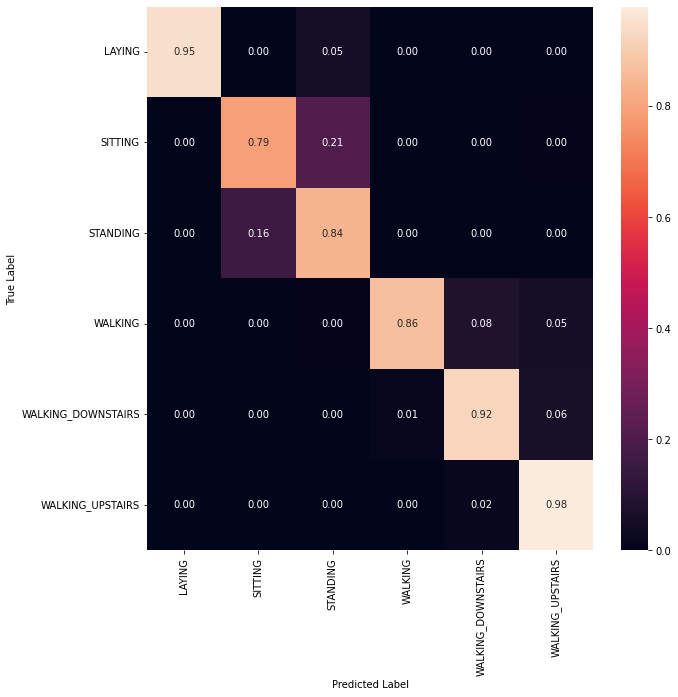
\includegraphics[width= 0.9 \linewidth]{LSTM(1)_Results.png}
	\centering
	\caption{LSTM Model Architecture 1 Results}
	\label{LSTM(1)_Results.png}
\end{figure}

Based on the Figure 17, which depicts the Confusion Matrix for LSTM Model Architecture 1, it is clear that this architecture performs decently well. What we can see is that this model, occasionally, gets mixed up between Standing and Sitting Down. This is quite understandable because when sitting down and standing up, the sensor readings will be roughly the same because both of the aforementioned activities are stationary activities. Hence, to try to get our model to better distinguish between these two activities, we tried two things. The first thing we tried was to increase the number of LSTM Layers. The second thing we tried was to add an Attention Layer to the model. 

\begin{figure}[h!]
	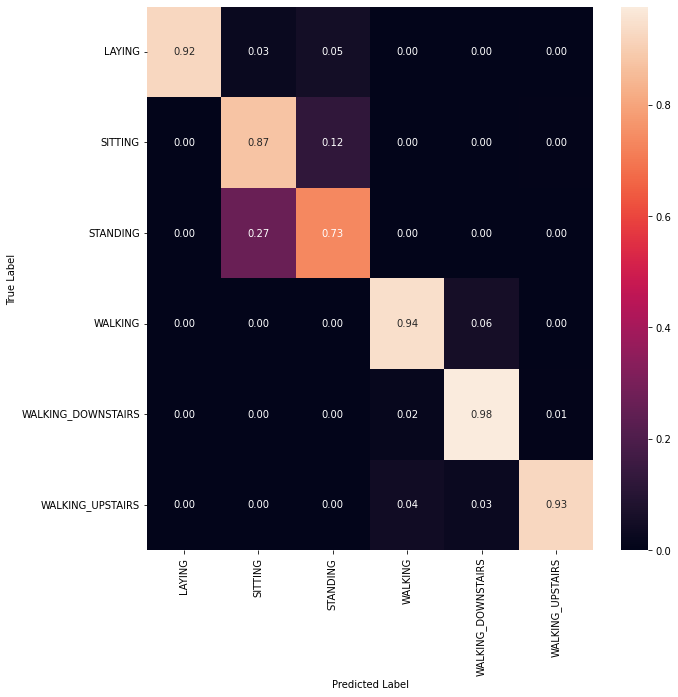
\includegraphics[width= 0.9 \linewidth]{LSTM(2)_Results.png}
	\centering
	\caption{LSTM Model Architecture 2 Results}
	\label{LSTM(2)_Results.png}
\end{figure}

Based on Figure 18, which depicts the Confusion Matrix for LSTM Model Architecture 2, Architecture 2 seemed to help the system correctly identify more samples where users were sitting. However, this system performs a bit worsely on samples where users are standing. Hence, this doesn't quite solve the problem. 



\begin{figure}[h!]
	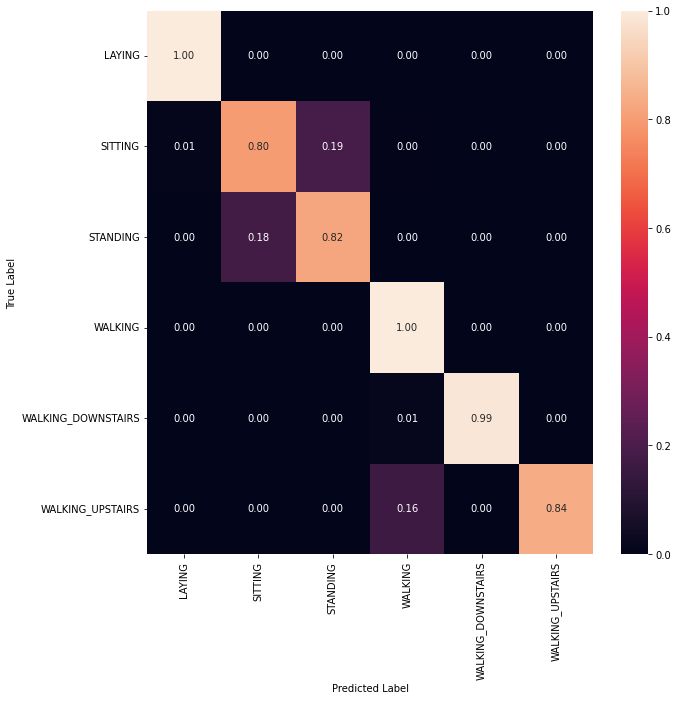
\includegraphics[width= 0.9 \linewidth]{LSTM(3)_Results.png}
	\centering
	\caption{LSTM Model Architecture 3 Results}
	\label{LSTM(3)_Results.png}
\end{figure}

Based on the Figure 19, which depicts the Confusion Matrix for LSTM Model Architecture 3, Architecture 3 didn't seem to offer much improvement over the Sitting vs Standing Dilemma. Additionally, it seemed to worsen the prediction accuracy for Walking Upstairs Cases. We believe this occurred because attention mechanisms, especially if the model is complex, can potentially lead to overfitting when the amount of data is limited. Our feeling is that the attention layer we had in this model did not generalize well. 

\begin{figure}
    \centering
    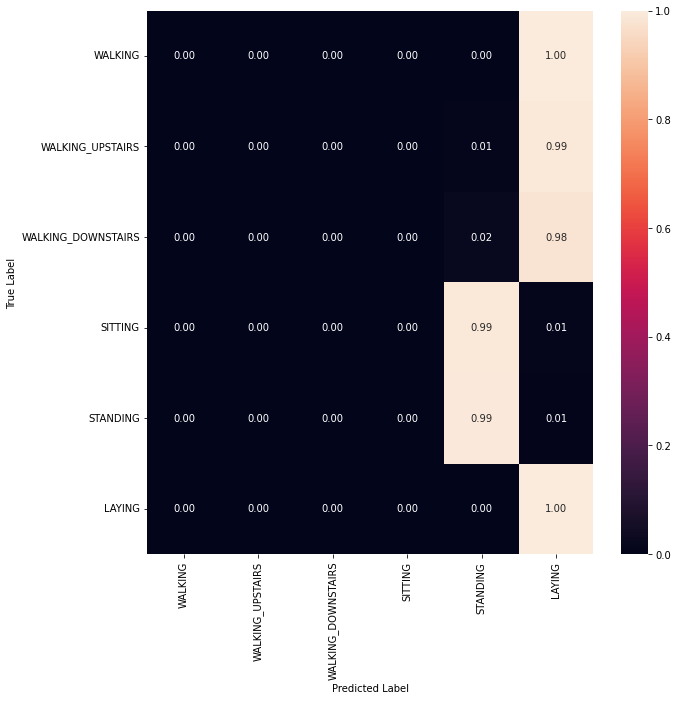
\includegraphics[width= 0.9 \linewidth]{transformer_results.png}
    \caption{Transformer Results}
    \label{transformer_results.png}
\end{figure}

Based on Figure 20, which depicts the Confusion Matrix for the Transformer, it is evident that the Transformer did not perform as well as the other models. We must remember that the major cavaeat with Transformer Models is that training Multi-Head Attention Layers within the Transformer Model often require a significant amount of data to converge to an optimal solution. In this dataset, we only have 30 subjects and overall roughly 7353 time series samples. Hence, we can say the amount of data is not enough to train the attention layer to converge to an optimal solution. 




\begin{figure}[h!]
    \centering
    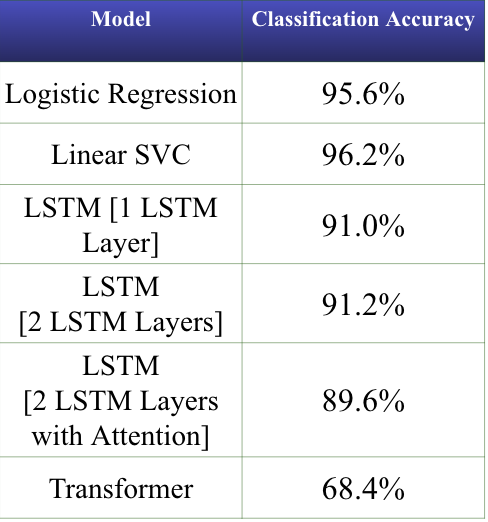
\includegraphics[width= 0.9 \linewidth]{results.png}
    \caption{Overall Accuracy Results}
    \label{results.png}
\end{figure}

Based on Figure 21, which shows the overall accuracy results for all of our models, it is clear to see that the Baseline Models outperformed the Deep Learning Models. However, it is key to note that Logistic Regression and Linear SVC followed a different training process than the LSTM Models and Transformer Model. First and foremost, the LSTM Models and Transformer Model were trained mainly on raw sensor data[Note: Acceleration Data was split into Body + Gravitational Acceleration via Low Pass Filtration]. On the other hand, the Logistic Regression and Linear SVC Models were trained on preprocessed data. \newline 

Finally, the results made it evident that, when we added attention layers to the LSTM Model, it made the accuracy worse. Furthermore, we can see that the Transformer had the lowest accuracy among all the models. As discussed earlier within this work, these observations are occurring, most likely, due to limited data to train all the attention layers.


\section{Conclusion and Future Work}
The unexpected performance of the Transformer model, which demonstrated the lowest accuracy among all models, could be attributed to its intricate architecture and the challenges associated with training attention layers effectively. Transformers are renowned for their success in processing sequential data, especially in natural language tasks. However, their performance can be contingent on the availability of an extensive dataset to train the numerous attention mechanisms effectively. In the context of our HAR dataset, the limited volume of data might have hindered the Transformer's ability to discern and learn the intricate patterns required for accurate activity recognition.

The superior performance of baseline models, such as Logistic Regression and Linear SVC, over Neural Network models raises questions about the interplay between model complexity and dataset characteristics. In scenarios with limited data or simpler underlying patterns, more complex models may struggle to generalize effectively. The baseline models, being less complex and more interpretable, might have exhibited better robustness in the face of these constraints.

The divergence in training processes between Neural Network models and baseline models further emphasizes the importance of data preprocessing. The Neural Network models, specifically LSTM and Transformer, leveraged raw sensor data, with an additional step of decomposing the acceleration data into Body and Gravitational components using low-pass filtration. This preprocessing step was tailored to enhance the model's ability to discern meaningful patterns in the data. On the other hand, the baseline models were trained on preprocessed data, potentially missing out on subtle features present in the raw sensor readings.

The direct correlation observed between the accuracy of the LSTM model and the number of LSTM/Attention Layers emphasizes the importance of model architecture. More complex models, with a greater number of layers, were better equipped to capture intricate temporal dependencies within sequential sensor data. This underscores the need for careful consideration of model architecture based on the nature of the data and the complexity of underlying patterns.

In considering future work, there are several avenues for exploration and improvement based on the insights gained from this analysis:

1. \textbf{Model Refinement:} Future research could focus on refining the architecture of the Transformer model, addressing the challenges associated with training attention layers effectively. This may involve experimenting with different configurations and techniques to enhance the model's performance on the specific nature of the Human Activity Recognition (HAR) dataset.

2. \textbf{Data Augmentation:} Given the limited volume of data in the HAR dataset, exploring data augmentation techniques could be beneficial. Augmenting the dataset with variations of existing samples could potentially improve the generalization ability of more complex models, such as the Transformer.

3. \textbf{Feature Engineering:} Investigating additional features or representations that capture subtle patterns in raw sensor readings might enhance the performance of baseline models. Feature engineering tailored to the unique characteristics of the dataset could contribute to better model understanding and accuracy.

4. \textbf{Ensemble Approaches:} Considering ensemble methods that combine predictions from multiple models may lead to improved overall performance. Combining the strengths of different models, especially baseline models and more complex neural network models, could mitigate the limitations of individual approaches.

5. \textbf{Data Diversity:} Collecting and incorporating additional diverse data into the HAR dataset may contribute to better model generalization. A more extensive and varied dataset could aid in training attention mechanisms effectively within complex models like the Transformer.

6. \textbf{Interpretability and Explainability:} Given the superior robustness exhibited by baseline models, future work could delve into enhancing the interpretability of more complex models. Developing methods to interpret and explain the decisions made by models like the Transformer may improve their trustworthiness in real-world applications.

By exploring these areas, researchers and practitioners can advance the field of Human Activity Recognition and tailor models to better meet the demands of real-world scenarios.

In conclusion, the unexpected findings underscore the nuanced relationship between model complexity, dataset characteristics, and preprocessing steps. The optimal choice of a model for HAR depends on the intricacies of the dataset, and the findings highlight the importance of aligning model selection with the specific requirements and constraints of the task at hand. The analysis provides valuable insights for researchers and practitioners in tailoring HAR systems to real-world scenarios, where data availability and interpretability are crucial considerations.


\section*{Acknowledgment}
We would like to thank Professor Jorge Ortiz for his continued support during the course of the Fall 2023 Semester. 

\begin{thebibliography}{00}
\bibitem{b1} Y. Shavit and I. Klein, "Boosting Inertial-Based Human Activity Recognition With Transformers," in IEEE Access, vol. 9, pp. 53540-53547, 2021, doi: 10.1109/ACCESS.2021.3070646.
\bibitem{b2} Messitte, N. (2023, January 6). 6 Ways to Use a Low Pass Filter When Mixing. iZotope. https://www.izotope.com/en/learn/6-ways-to-use-a-low-pass-filter-when-mixing.html.
\bibitem{b3} Nafea O, Abdul W, Muhammad G, Alsulaiman M. Sensor-Based Human Activity Recognition with Spatio-Temporal Deep Learning. Sensors. 2021; 21(6):2141. https://doi.org/10.3390/s21062141.
\bibitem{b4} Vaswani, A., Shazeer, N., Parmar, N., Uszkoreit, J., Jones, L., Gomez, A. N., Kaiser, L., \&; Polosukhin, I. (2023, August 2). Attention is all you need. arXiv.org. https://doi.org/10.48550/arXiv.1706.03762.
\bibitem{b5} Jorge-L. Reyes-Ortiz, Luca Oneto, Albert Samà, Xavier Parra, Davide Anguita, Transition-Aware Human Activity Recognition Using Smartphones, Neurocomputing, Volume 171, 2016, Pages 754-767, ISSN 0925-2312, https://doi.org/10.1016/j.neucom.2015.07.085.
\bibitem{b6} Charissa Ann Ronao, Sung-Bae Cho,
Human activity recognition with smartphone sensors using deep learning neural networks, Expert Systems with Applications, Volume 59, 2016, Pages 235-244, ISSN 0957-4174, https://doi.org/10.1016/j.eswa.2016.04.032.
\end{thebibliography}
\vspace{12pt}
\end{document}
